\chapter{The IMU}
\label{ch:imu}

A camera fails in exactly the situations a mower meets every day: when
it faces a uniform wall of hedge, when it turns quickly at the end of a
row, when the sun shines straight into the lens, when the deck vibrates.
An inertial measurement unit (IMU) does not care about any of this. It
measures the angular rate and the acceleration of the body two hundred
times per second or more, and those can be integrated into motion. But
the integration drifts: within half a minute an IMU alone has lost the
mower by metres. Vision and inertia are complementary, and Part~IV is
about fusing them with the other sensors of the garden. This chapter
prepares the inertial side: what an IMU measures, how its errors are
characterised, how its measurements are integrated on $\SO3$, and how the
hundreds of samples between two keyframes are condensed into a single
factor for the optimisation of Chapter~13 --- \emph{preintegration}.

Notation for the whole of Part~IV:
\begin{itemize}[nosep]
\item the world frame $W$ has $z$ up, and gravity is
  $\vect{g}=(0,0,-9.81)$\,m/s$^2$;
\item the body (IMU) frame $B$ has pose $(R,\p)$ with $R=R_{WB}$, and
  velocity $\vect{v}$ in $W$;
\item perturbations are on the right as in Chapter~\ref{ch:rigid}:
  $R\leftarrow R\Exp(\delta\bphi)$,
  $\vect{v}\leftarrow\vect{v}+\delta\vect{v}$ and
  $\p\leftarrow\p+R\,\delta\p$.
\end{itemize}

\section{What an IMU measures}

A MEMS IMU contains a three-axis gyroscope and a three-axis
accelerometer. The accelerometer does not measure acceleration: it
measures the force per unit mass needed to keep its proof mass in
place, that is acceleration \emph{minus gravity}. An accelerometer
resting on a table therefore reads $+9.81$\,m/s$^2$ upwards, and one in
free fall reads zero.

\begin{definition}{IMU measurement model}{imumodel}
At time $t$ the IMU returns
\begin{equation}\label{eq:imumodel}
\tilde{\bomega}=\bomega+\vect{b}_g+\vect{\eta}_g,\qquad
\tilde{\vect{a}}=R\T(\vect{a}-\vect{g})+\vect{b}_a+\vect{\eta}_a,
\end{equation}
where $\bomega$ is the angular rate in the body frame, $\vect{a}=\ddot\p$
the acceleration in the world frame, $\vect{b}_g,\vect{b}_a$ slowly
varying biases, and $\vect{\eta}_g,\vect{\eta}_a$ white noise. The
quantity $R\T(\vect{a}-\vect{g})$ is the \emph{specific force}. The
biases follow random walks, $\dot{\vect{b}}_g=\vect{\eta}_{bg}$,
$\dot{\vect{b}}_a=\vect{\eta}_{ba}$.
\end{definition}

The model leaves out the rotation of the Earth ($7.3\times10^{-5}$\,rad/s,
$15^\circ$/h), which is below the bias uncertainty of consumer MEMS
gyroscopes. It also leaves out scale factors, misalignment between axes,
sensitivity of the gyroscope to acceleration, and the dependence of
everything on temperature. A factory or Allan-style calibration takes
care of the first ones, and the bias random walk partly absorbs the
rest. The position of the IMU relative to the camera, and the time
offset between the two, matter as much as the noise; they are
Chapter~13's business.

\section{Noise, and how to measure it}

White noise in continuous time has infinite variance. What is specified
is its \emph{density} $\sigma$, such that its integral over an interval
of length $\Delta t$ has variance $\sigma^2\Delta t$. Gyroscope densities
are given in rad/s/$\sqrt{\text{Hz}}$ (or as an \emph{angle random walk}
in $^\circ/\sqrt{\text{h}}$), accelerometer densities in
m/s$^2$/$\sqrt{\text{Hz}}$ (or $\mu g/\sqrt{\text{Hz}}$).

\begin{proposition}{Discrete-time noise}{discnoise}
A sensor whose output is white noise of density $\sigma$, averaged over a
sampling interval $\Delta t$, delivers samples with standard deviation
$\sigma/\sqrt{\Delta t}$. A random walk driven by white noise of density
$\sigma_b$ changes between two samples by a Gaussian increment of
standard deviation $\sigma_b\sqrt{\Delta t}$.
\end{proposition}

\begin{proof}
Write the noise as $\sigma\,\dot W$ with $W$ a standard Wiener process.
The average over the interval is $\frac{\sigma}{\Delta t}(W(t+\Delta t)-
W(t))$, of variance $\sigma^2\Delta t/\Delta t^2=\sigma^2/\Delta t$. The
random walk $\sigma_bW$ changes by $\sigma_b(W(t+\Delta t)-W(t))$, of
variance $\sigma_b^2\Delta t$.
\end{proof}

At 200\,Hz, the gyroscope of the EuRoC dataset (an ADIS16448, density
$1.7\times10^{-4}$\,rad/s/$\sqrt{\text{Hz}}$) has per-sample noise of
$2.4\times10^{-3}$\,rad/s, $0.14^\circ$/s. The noise of a sample
depends on the rate; the density does not, which is why datasheets give
the density.

How are $\sigma$ and $\sigma_b$ measured? Leave the IMU still for a few
hours and compute its \emph{Allan variance}.

\begin{definition}{Allan variance}{allan}
Let $y(t)$ be a sensor output and $\bar y_k(\tau)=\frac1\tau
\int_{k\tau}^{(k+1)\tau}y(t)\,dt$ its averages over consecutive
intervals of length $\tau$. The Allan variance is
\begin{equation}\label{eq:allan}
\sigma_A^2(\tau)=\tfrac12\,\E\bigl[(\bar y_{k+1}(\tau)-\bar y_k(\tau))^2
\bigr],
\end{equation}
and $\sigma_A(\tau)$ the Allan deviation.
\end{definition}

Differencing successive averages removes any constant value, so a
constant bias does not contribute. Each noise process leaves its own
signature as a function of $\tau$.

\begin{proposition}{Allan variance of white noise and of a random
walk}{allanforms}
For white noise of density $\sigma$, $\sigma_A^2(\tau)=\sigma^2/\tau$.
For a random walk driven by white noise of density $\sigma_b$,
$\sigma_A^2(\tau)=\sigma_b^2\tau/3$. For independent processes the Allan
variances add.
\end{proposition}

\begin{proof}
White noise: $\bar y_k$ and $\bar y_{k+1}$ are averages over disjoint
intervals, hence independent, each of variance $\sigma^2/\tau$
(\cref{prop:discnoise}); their difference has variance $2\sigma^2/\tau$.

Random walk: $y=\sigma_bW$. Then
\[
\bar y_{k+1}-\bar y_k=\frac{\sigma_b}\tau\int_0^\tau\bigl(W(s+\tau)-
W(s)\bigr)ds=\frac{\sigma_b}\tau\int_0^\tau\!\!\int_s^{s+\tau}dW(u)\,ds
=\frac{\sigma_b}\tau\int_0^{2\tau}\kappa(u)\,dW(u),
\]
taking $k=0$ without loss of generality and exchanging the integrals,
where $\kappa(u)$ is the length of $\{s\in[0,\tau]:s\le u\le s+\tau\}$:
$\kappa(u)=u$ on $[0,\tau]$ and $2\tau-u$ on $[\tau,2\tau]$. By the
It\^o isometry the variance is $\frac{\sigma_b^2}{\tau^2}\int_0^{2\tau}
\kappa(u)^2du=\frac{\sigma_b^2}{\tau^2}\cdot2\cdot\frac{\tau^3}3=
\frac23\sigma_b^2\tau$. Halving gives $\sigma_b^2\tau/3$.

Additivity: for $y=y_1+y_2$ independent and zero-mean, the cross term of
$\E[(\Delta\bar y_1+\Delta\bar y_2)^2]$ vanishes.
\end{proof}

On a log--log plot of $\sigma_A$, white noise is a line of slope
$-\frac12$ that passes through $\sigma$ at $\tau=1$\,s, and a bias random
walk is a line of slope $+\frac12$ that passes through $\sigma_b$ at
$\tau=3$\,s. Real sensors also show a flat region between the two, the
\emph{bias instability}, caused by flicker noise that no finite set of
white and random-walk terms reproduces exactly. Our model has no such
term, and filters and optimisers usually do not model it either; it is
absorbed by inflating $\sigma_b$.

\begin{figure}[ht]
\centering
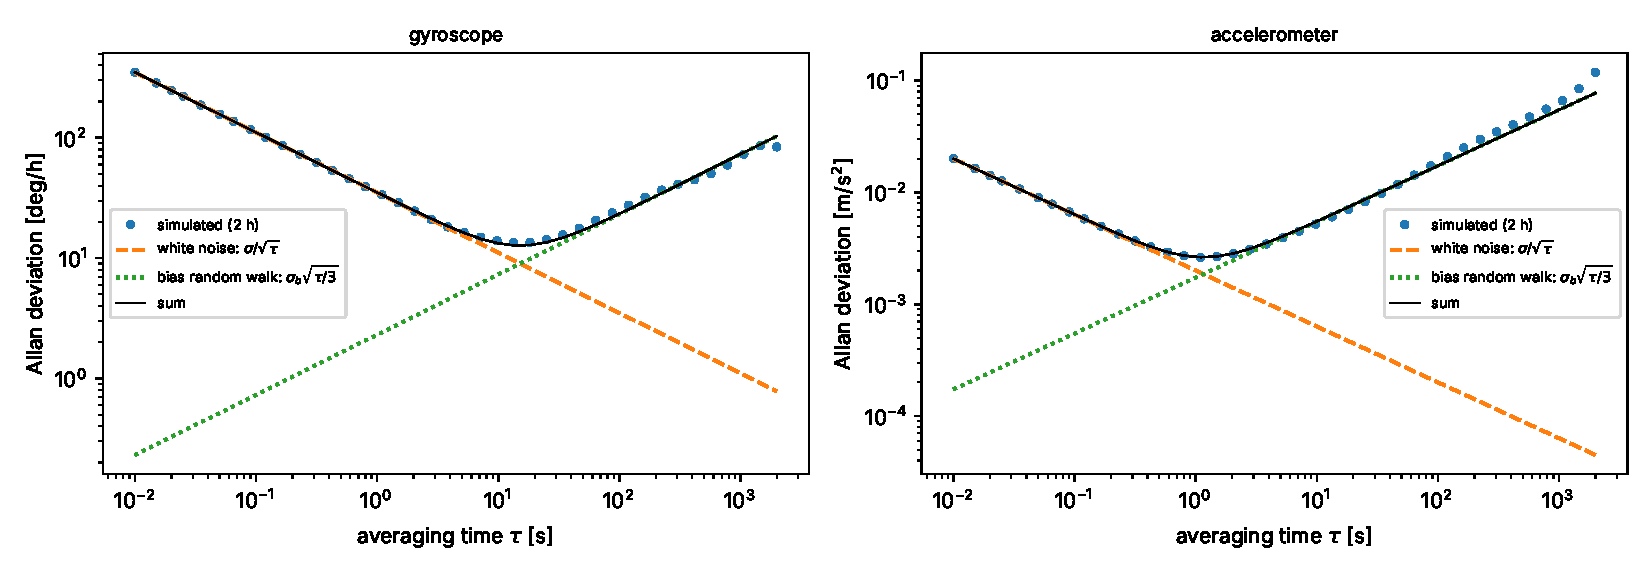
\includegraphics[width=\linewidth]{figures/ch12_allan.pdf}
\caption{Allan deviations of two hours of a simulated stationary IMU
with the EuRoC noise parameters, against \cref{prop:allanforms}. The
curves cross at $\tau^*=\sqrt3\,\sigma/\sigma_b$: 15\,s for the
gyroscope, 1.2\,s for the accelerometer. The scatter at long $\tau$
comes from the few independent averages left.}
\label{fig:allan}
\end{figure}

\Cref{fig:allan} also shows a trap. For the accelerometer the two lines
cross near 1\,s, so reading the white-noise density at $\tau=1$\,s gives
$2.6\times10^{-3}$ instead of $2.0\times10^{-3}$: both slopes must be
fitted. Tools such as \code{allan\_variance\_ros} or Kalibr's
\code{imu\_utils} do this on a recording of a few hours.

\section{Kinematics and strapdown integration}

The state $(R,\vect{v},\p)$ evolves as
\begin{equation}\label{eq:imukin}
\dot R=R\,\hatop{\bomega},\qquad\dot{\vect{v}}=\vect{a}=
R(\tilde{\vect{a}}-\vect{b}_a-\vect{\eta}_a)+\vect{g},\qquad
\dot\p=\vect{v},
\end{equation}
with $\bomega=\tilde\bomega-\vect{b}_g-\vect{\eta}_g$. Integrating these
equations with the measurements is called \emph{strapdown} integration
(the sensors are strapped to the body, not on a stabilised platform).

\begin{lemma}{One integration step}{imustep}
If $\bomega$ is constant on $[t,t+\Delta t]$, then $R(t+\Delta t)=R(t)
\Exp(\bomega\Delta t)$ exactly. If moreover the specific force is
constant and $R$ is replaced by $R(t)$ on the interval, then
\begin{equation}\label{eq:imustep}
\vect{v}(t+\Delta t)=\vect{v}+\vect{a}\Delta t,\qquad
\p(t+\Delta t)=\p+\vect{v}\Delta t+\tfrac12\vect{a}\Delta t^2,\qquad
\vect{a}=R(t)\tilde{\vect{a}}'+\vect{g},
\end{equation}
with $\tilde{\vect{a}}'$ the bias-corrected specific force; the error of
this approximation is of order $\Delta t^2$ per step.
\end{lemma}

\begin{proof}
With $\bomega$ constant, $\dot R=R\hatop{\bomega}$ is a linear ODE with a
constant matrix, whose solution is $R(t)\exp(\hatop{\bomega}(s-t))$
(\cref{lem:dexp}). For the velocity, $\vect{a}(s)=R(s)\tilde{\vect{a}}'
+\vect{g}$ and $R(s)=R(t)+O(s-t)$, so $\int_t^{t+\Delta t}\vect{a}=
\vect{a}(t)\Delta t+O(\Delta t^2)$; the position is the same with one
more integration.
\end{proof}

Over $n=T/\Delta t$ steps the errors of order $\Delta t^2$ add up to an
error of order $\Delta t$: the scheme is first order. Its velocity
error over an interval is about $\frac12\Delta t$ times the change of
the acceleration in that interval, which at 200\,Hz on a mower is
comparable to the noise (\cref{fig:imubias}, right). Higher-order
schemes exist (midpoint integration, closed-form preintegration); this
one is what most systems and GTSAM use.

How fast does the integration drift? The next proposition linearises
the errors for a level IMU at rest, which is also what governs a slowly
moving mower.

\begin{proposition}{Strapdown drift}{drift}
Consider a level IMU at rest whose integration starts with the exact
state. Along one horizontal axis, an accelerometer bias error $\delta
b_a$, a gyroscope bias error $\delta b_g$ (about the perpendicular
horizontal axis), and white noises of densities $\sigma_a$, $\sigma_g$
produce, to first order, the position error
\begin{equation}\label{eq:drift}
\delta p(t)=\tfrac12\delta b_a\,t^2+\tfrac16\,g\,\delta b_g\,t^3+
\epsilon(t),\qquad
\E\,\epsilon(t)^2=\frac{\sigma_a^2t^3}3+\frac{g^2\sigma_g^2t^5}{20}.
\end{equation}
\end{proposition}

\begin{proof}
A tilt error $\delta\theta$ about the perpendicular horizontal axis makes
the integration project gravity onto the axis: $g\,\delta\theta$ (up to
a sign fixed by the axes, which the variance and the magnitudes do not
see). The errors therefore obey $\delta\dot\theta=\delta b_g+\eta_g$,
$\delta\ddot p=g\,\delta\theta+\delta b_a+\eta_a$, all starting at zero.
Hence $\delta\theta(s)=\delta b_g\,s+\int_0^s\eta_g$, and integrating
twice, $\delta p(t)=\int_0^t(t-s)\bigl(g\,\delta\theta(s)+\delta b_a+
\eta_a(s)\bigr)ds$. The deterministic terms give $\frac12\delta b_at^2$
and $g\,\delta b_g\int_0^t(t-s)s\,ds=g\,\delta b_gt^3/6$. The
accelerometer noise gives $\int_0^t(t-s)\eta_a(s)ds$, of variance
$\sigma_a^2\int_0^t(t-s)^2ds=\sigma_a^2t^3/3$. The gyroscope noise gives
$g\int_0^t(t-s)\sigma_gW(s)ds$, of variance $g^2\sigma_g^2\int_0^t\!\int_0^t
(t-s)(t-u)\min(s,u)\,du\,ds$; by symmetry this is twice the integral
over $u<s$:
\[
2\int_0^t(t-s)\int_0^s(t-u)u\,du\,ds
=2\int_0^t(t-s)\Bigl(\frac{ts^2}2-\frac{s^3}3\Bigr)ds
=2\Bigl(\frac{t^5}6-\frac{t^5}{12}-\frac{t^5}{8}+\frac{t^5}{15}\Bigr)
=\frac{t^5}{20}.
\]
The two noises are independent, so their variances add.
\end{proof}

\begin{figure}[ht]
\centering
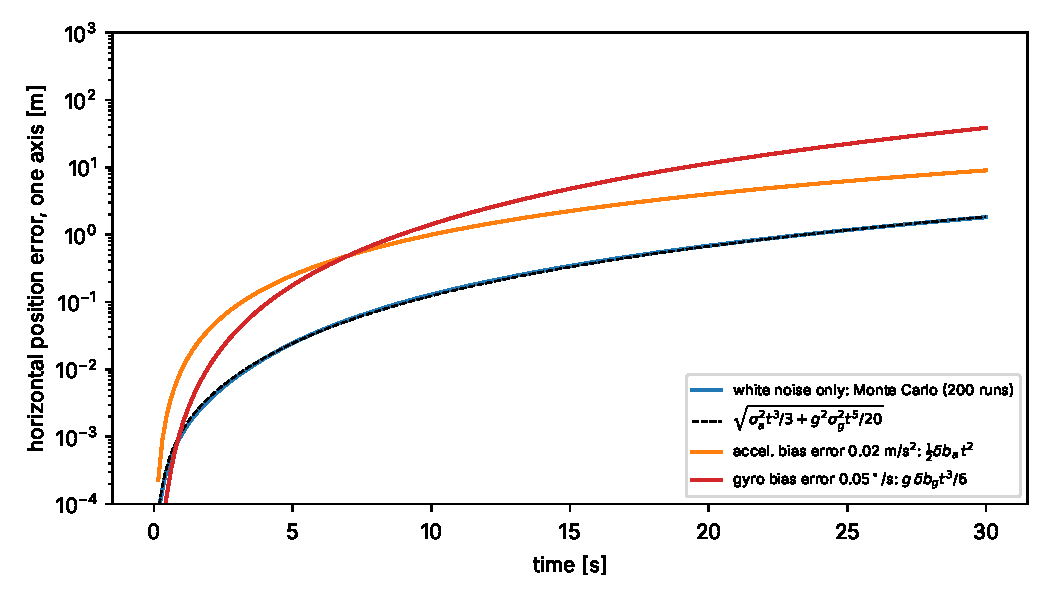
\includegraphics[width=0.78\linewidth]{figures/ch12_drift.pdf}
\caption{Dead reckoning with the EuRoC IMU. Blue: position error of a
level IMU at rest with exactly known biases (200 Monte Carlo runs),
against \eqref{eq:drift}. Orange and red: the effect of small bias
errors alone.}
\label{fig:drift}
\end{figure}

\begin{inwords}
Inertial errors grow like powers of time, and the gyroscope dominates
through gravity: a tilt error of a fraction of a degree projects a
fraction of $9.81$\,m/s$^2$ onto the horizontal, which is then
integrated twice. With the EuRoC IMU and biases known exactly, the
noise alone costs 12\,cm after 10\,s and 1.8\,m after 30\,s; a gyro
bias error of $0.05^\circ$/s, small next to the turn-on bias of a
consumer gyroscope, costs 1.4\,m after 10\,s and 39\,m after 30\,s. An IMU
alone cannot localise a mower. Over the 0.1--0.5\,s between two
keyframes, though, it is excellent, and that is how it will be used.
\end{inwords}

\section{Preintegration}

Visual--inertial optimisation (Chapter~13) estimates the states
$(R,\vect{v},\p,\vect{b}_g,\vect{b}_a)$ of the keyframes only; between
keyframes $i$ and $j$ lie tens or hundreds of IMU samples. They must
become one factor linking the two states. Integrating them in the world
frame would need $R_i$ and $\vect{v}_i$, so every iteration that moves
$R_i$ would require integrating them again. Preintegration removes this
dependence by integrating in the frame of keyframe $i$ and pulling
gravity out.

\begin{theorem}{Preintegrated measurements}{preint}
Let samples $k=i,\dots,j-1$ have period $\Delta t$, let $\Delta t_{ij}=
(j-i)\Delta t$, fix biases $\vect{b}_g,\vect{b}_a$, and write
$\bomega_k=\tilde\bomega_k-\vect{b}_g$, $\vect{f}_k=\tilde{\vect{a}}_k-
\vect{b}_a$. Define
\begin{equation}\label{eq:preint}
\Delta R_{ij}=\prod_{k=i}^{j-1}\Exp(\bomega_k\Delta t),\quad
\Delta\vect{v}_{ij}=\sum_{k=i}^{j-1}\Delta R_{ik}\vect{f}_k\Delta t,\quad
\Delta\p_{ij}=\sum_{k=i}^{j-1}\Bigl(\Delta\vect{v}_{ik}\Delta t+
\tfrac12\Delta R_{ik}\vect{f}_k\Delta t^2\Bigr),
\end{equation}
with $\Delta R_{ii}=I$, $\Delta\vect{v}_{ii}=\Delta\p_{ii}=\vect{0}$.
If the states follow the integration of \cref{lem:imustep} with these
samples, then
\begin{equation}\label{eq:preintrel}
\begin{aligned}
R_j&=R_i\,\Delta R_{ij},\\
\vect{v}_j&=\vect{v}_i+\vect{g}\Delta t_{ij}+R_i\,\Delta\vect{v}_{ij},\\
\p_j&=\p_i+\vect{v}_i\Delta t_{ij}+\tfrac12\vect{g}\Delta t_{ij}^2+
R_i\,\Delta\p_{ij}.
\end{aligned}
\end{equation}
\end{theorem}

\begin{proof}
By induction on $j$. For $j=i$, \eqref{eq:preintrel} holds trivially.
Suppose it holds for $j$, and write $\vect{f}=\vect{f}_j$, $\tau=\Delta t$.
Then $R_{j+1}=R_j\Exp(\bomega_j\tau)=R_i\Delta R_{ij}\Exp(\bomega_j\tau)
=R_i\Delta R_{i,j+1}$. Next,
\[
\vect{v}_{j+1}=\vect{v}_j+(R_j\vect{f}+\vect{g})\tau
=\vect{v}_i+\vect{g}(\Delta t_{ij}+\tau)+R_i\bigl(\Delta\vect{v}_{ij}+
\Delta R_{ij}\vect{f}\tau\bigr),
\]
and the bracket is $\Delta\vect{v}_{i,j+1}$. Finally,
\[
\begin{aligned}
\p_{j+1}&=\p_j+\vect{v}_j\tau+\tfrac12(R_j\vect{f}+\vect{g})\tau^2\\
&=\p_i+\vect{v}_i(\Delta t_{ij}+\tau)
+\tfrac12\vect{g}\bigl(\Delta t_{ij}^2+2\Delta t_{ij}\tau+\tau^2\bigr)
+R_i\bigl(\Delta\p_{ij}+\Delta\vect{v}_{ij}\tau+\tfrac12\Delta R_{ij}
\vect{f}\tau^2\bigr),
\end{aligned}
\]
in which $\Delta t_{ij}^2+2\Delta t_{ij}\tau+\tau^2=\Delta t_{i,j+1}^2$
and the last bracket is $\Delta\p_{i,j+1}$.
\end{proof}

The preintegrated measurements depend on the IMU samples and the biases
only, not on the states. They are computed once, recursively, as the
samples arrive: $\Delta\p$ first (it needs $\Delta\vect{v}_{ij}$ and
$\Delta R_{ij}$ before they are updated), then $\Delta\vect{v}$, then
$\Delta R$. Read in the other direction, \eqref{eq:preintrel} says what
the measurements should be for given states:
\begin{equation}\label{eq:preintinv}
\Delta R_{ij}=R_i\T R_j,\quad
\Delta\vect{v}_{ij}=R_i\T(\vect{v}_j-\vect{v}_i-\vect{g}\Delta t_{ij}),\quad
\Delta\p_{ij}=R_i\T\bigl(\p_j-\p_i-\vect{v}_i\Delta t_{ij}-\tfrac12
\vect{g}\Delta t_{ij}^2\bigr).
\end{equation}
This is the measurement model of the IMU factor. What remains is its
uncertainty, and what happens when the biases change.

\section{The noise of preintegrated measurements}

Three first-order identities on $\SO3$ do all the work. For small
$\vect{x}$, $\vect{y}$:
\begin{equation}\label{eq:so3id}
\Exp(\bphi+\vect{x})\approx\Exp(\bphi)\Exp(J_r(\bphi)\vect{x}),\quad
\Exp(\vect{x})R=R\Exp(R\T\vect{x}),\quad
\Exp(\vect{x})\Exp(\vect{y})\approx\Exp(\vect{x}+\vect{y}).
\end{equation}
The first is the definition of the right Jacobian (\cref{thm:jr}). The
second is exact, since by \cref{lem:hatid}~(v)
\[
R\Exp(R\T\vect{x})R\T=\exp\bigl(R\,\hatop{(R\T\vect{x})}\,R\T\bigr)
=\exp(\hatop{\vect{x}})=\Exp(\vect{x}).
\]
The third holds up to second-order terms.

\begin{proposition}{Noise propagation}{preintnoise}
Let the samples carry noise, $\tilde\bomega_k=\bomega_k+\vect{b}_g+
\vect{\eta}_{g,k}$ and $\tilde{\vect{a}}_k=\vect{f}_k+\vect{b}_a+
\vect{\eta}_{a,k}$ with independent $\vect\eta_{g,k}\sim\Normal(0,
\frac{\sigma_g^2}{\Delta t}I)$ and $\vect\eta_{a,k}\sim\Normal(0,
\frac{\sigma_a^2}{\Delta t}I)$ (\cref{prop:discnoise}). Let $\Delta
\tilde R_{ij},\Delta\tilde{\vect{v}}_{ij},\Delta\tilde\p_{ij}$ be
\eqref{eq:preint} computed from the noisy samples and $\Delta R_{ij},
\Delta\vect{v}_{ij},\Delta\p_{ij}$ from the noise-free ones. Define the
errors $\delta\bphi_{ij},\delta\vect{v}_{ij},\delta\p_{ij}$ by
\begin{equation}\label{eq:preinterr}
\Delta\tilde R_{ij}=\Delta R_{ij}\Exp(\delta\bphi_{ij}),\quad
\Delta\tilde{\vect{v}}_{ij}=\Delta\vect{v}_{ij}+\delta\vect{v}_{ij},\quad
\Delta\tilde\p_{ij}=\Delta\p_{ij}+\delta\p_{ij}.
\end{equation}
To first order, $\vect{e}_{ij}=(\delta\bphi_{ij},\delta\vect{v}_{ij},
\delta\p_{ij})$ obeys $\vect{e}_{ii}=\vect{0}$ and
$\vect{e}_{i,j+1}=A_j\vect{e}_{ij}+B_j\vect{n}_j$ with
$\vect{n}_j=(\vect\eta_{g,j},\vect\eta_{a,j})$ and, writing $\tau=\Delta
t$, $\tilde{\vect{f}}=\tilde{\vect{a}}_j-\vect{b}_a$ and $\Delta
\tilde R_{j,j+1}=\Exp((\tilde\bomega_j-\vect{b}_g)\tau)$,
\begin{equation}\label{eq:preintAB}
A_j=\begin{pmatrix}\Delta\tilde R_{j,j+1}\T&0&0\\
-\Delta\tilde R_{ij}\hatop{\tilde{\vect{f}}}\tau&I&0\\
-\frac12\Delta\tilde R_{ij}\hatop{\tilde{\vect{f}}}\tau^2&I\tau&I
\end{pmatrix},\quad
B_j=\begin{pmatrix}J_r^j\tau&0\\0&\Delta\tilde R_{ij}\tau\\
0&\frac12\Delta\tilde R_{ij}\tau^2\end{pmatrix},
\end{equation}
where $J_r^j=J_r((\tilde\bomega_j-\vect{b}_g)\tau)$. Hence the
covariance obeys $\Sigma_{i,j+1}=A_j\Sigma_{ij}A_j\T+B_jQB_j\T$,
$Q=\diag(\frac{\sigma_g^2}{\Delta t}I_3,\frac{\sigma_a^2}{\Delta t}I_3)$.
\end{proposition}

\begin{proof}
\emph{Rotation.} Let $\tilde{\vect{w}}_k=(\tilde\bomega_k-\vect{b}_g)
\tau$. By the first identity \eqref{eq:so3id}, each noise-free factor
is
\[
\Exp(\tilde{\vect{w}}_k-\vect\eta_{g,k}\tau)\approx
\Exp(\tilde{\vect{w}}_k)\Exp(-J_r^k\vect\eta_{g,k}\tau).
\] Write
$\vect{x}_k=J_r^k\vect\eta_{g,k}\tau$. Then
\[
\Delta R_{i,j+1}=\Delta R_{ij}\Exp(\tilde{\vect{w}}_j)\Exp(-\vect{x}_j)
=\Delta\tilde R_{ij}\Exp(-\delta\bphi_{ij})\Delta\tilde R_{j,j+1}
\Exp(-\vect{x}_j),
\]
using \eqref{eq:preinterr} for $j$. Moving $\Delta\tilde R_{j,j+1}$ to
the left with the second identity and merging with the third,
$\Delta R_{i,j+1}\approx\Delta\tilde R_{i,j+1}\Exp\bigl(-(\Delta\tilde
R_{j,j+1}\T\delta\bphi_{ij}+\vect{x}_j)\bigr)$, so
$\delta\bphi_{i,j+1}=\Delta\tilde R_{j,j+1}\T\delta\bphi_{ij}+J_r^j
\vect\eta_{g,j}\tau$.

\emph{Velocity.} The noise-free increment is $\Delta R_{ij}(\tilde{\vect{f}}
-\vect\eta_{a,j})\tau$ with $\Delta R_{ij}=\Delta\tilde R_{ij}
\Exp(-\delta\bphi_{ij})\approx\Delta\tilde R_{ij}(I-\hatop{\delta
\bphi_{ij}})$. To first order,
\[
\Delta R_{ij}(\tilde{\vect{f}}-\vect\eta_{a,j})\tau\approx
\Delta\tilde R_{ij}\tilde{\vect{f}}\tau
+\Delta\tilde R_{ij}\hatop{\tilde{\vect{f}}}\delta\bphi_{ij}\tau
-\Delta\tilde R_{ij}\vect\eta_{a,j}\tau ,
\]
using $-\hatop{\delta\bphi}\tilde{\vect{f}}=\hatop{\tilde{\vect{f}}}\delta
\bphi$. The noisy increment is $\Delta\tilde R_{ij}\tilde{\vect{f}}\tau$,
so $\delta\vect{v}_{i,j+1}=\delta\vect{v}_{ij}-\Delta\tilde R_{ij}
\hatop{\tilde{\vect{f}}}\delta\bphi_{ij}\tau+\Delta\tilde R_{ij}
\vect\eta_{a,j}\tau$.

\emph{Position.} In the same way, the increment
$\Delta\vect{v}_{ij}\tau+\frac12\Delta R_{ij}\vect{f}\tau^2$ gives
$\delta\p_{i,j+1}=\delta\p_{ij}+\delta\vect{v}_{ij}\tau-\frac12
\Delta\tilde R_{ij}\hatop{\tilde{\vect{f}}}\delta\bphi_{ij}\tau^2+
\frac12\Delta\tilde R_{ij}\vect\eta_{a,j}\tau^2$.

These three lines are $A_j\vect{e}_{ij}+B_j\vect{n}_j$ (the sign of the
noise terms does not affect the covariance). $\vect{n}_j$ is
independent of $\vect{e}_{ij}$, which depends on earlier samples only,
so the covariance propagates as stated.
\end{proof}

\begin{figure}[ht]
\centering
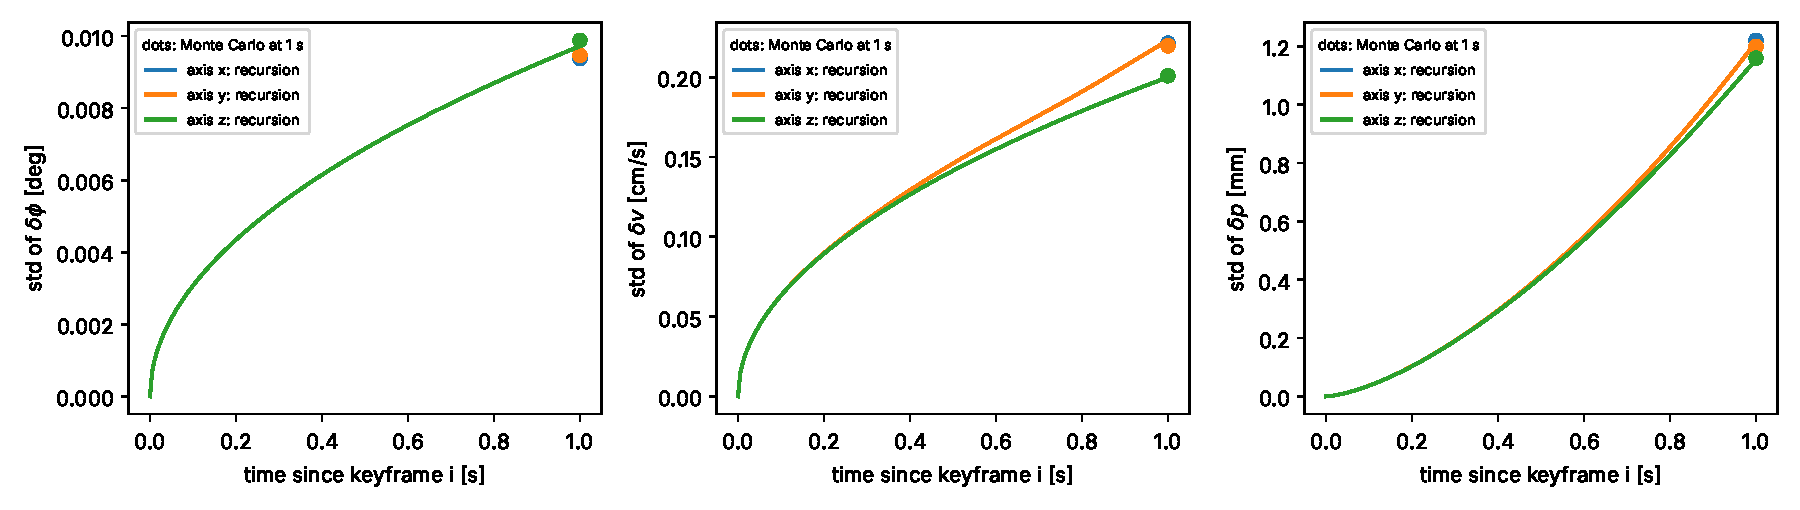
\includegraphics[width=\linewidth]{figures/ch12_preint.pdf}
\caption{Standard deviations of the preintegration errors along one
second of the lawn trajectory (driving along a row over bumps), from the
recursion of \cref{prop:preintnoise}, and from 1000 Monte Carlo runs at
the end (dots). They agree within 4\,\%.}
\label{fig:preint}
\end{figure}

\section{When the biases change}

The measurements \eqref{eq:preint} were computed with linearisation
biases $\bar{\vect{b}}_g,\bar{\vect{b}}_a$. The optimiser will move the
biases, and integrating again at every iteration is what preintegration
was meant to avoid. A first-order correction suffices.

\begin{proposition}{Bias Jacobians}{preintbias}
For $\vect{b}=\bar{\vect{b}}+\delta\vect{b}$, to first order,
\begin{equation}\label{eq:biasupd}
\begin{aligned}
\Delta R_{ij}(\vect{b})&\approx\Delta R_{ij}(\bar{\vect{b}})\Exp\bigl(
J^R_{ij}\delta\vect{b}_g\bigr),\\
\Delta\vect{v}_{ij}(\vect{b})&\approx\Delta\vect{v}_{ij}(\bar{\vect{b}})+
J^{v,g}_{ij}\delta\vect{b}_g+J^{v,a}_{ij}\delta\vect{b}_a,\\
\Delta\p_{ij}(\vect{b})&\approx\Delta\p_{ij}(\bar{\vect{b}})+
J^{p,g}_{ij}\delta\vect{b}_g+J^{p,a}_{ij}\delta\vect{b}_a,
\end{aligned}
\end{equation}
where the Jacobians start at zero and are updated with each sample, with
the quantities of \cref{prop:preintnoise} at $\bar{\vect{b}}$, by
\begin{equation}\label{eq:biasrec}
\begin{aligned}
J^R_{i,j+1}&=\Delta R_{j,j+1}\T J^R_{ij}-J_r^j\tau,&
J^{v,a}_{i,j+1}&=J^{v,a}_{ij}-\Delta R_{ij}\tau,\\
J^{v,g}_{i,j+1}&=J^{v,g}_{ij}-\Delta R_{ij}\hatop{\vect{f}}J^R_{ij}\tau,&
J^{p,a}_{i,j+1}&=J^{p,a}_{ij}+J^{v,a}_{ij}\tau-\tfrac12\Delta R_{ij}\tau^2,
\\
J^{p,g}_{i,j+1}&=J^{p,g}_{ij}+J^{v,g}_{ij}\tau-\tfrac12\Delta R_{ij}
\hatop{\vect{f}}J^R_{ij}\tau^2 .
\end{aligned}
\end{equation}
\end{proposition}

\begin{proof}
Changing the biases by $\delta\vect{b}$ changes every bias-corrected
sample exactly as noise $\vect\eta_{g,k}=\delta\vect{b}_g$,
$\vect\eta_{a,k}=\delta\vect{b}_a$ would: the measurements at
$\vect{b}$ are the ``noise-free'' ones of \cref{prop:preintnoise} and
those at $\bar{\vect{b}}$ the ``noisy'' ones. Hence $\Delta R_{ij}(
\vect{b})=\Delta R_{ij}(\bar{\vect{b}})\Exp(-\delta\bphi_{ij})$,
$\Delta\vect{v}_{ij}(\vect{b})=\Delta\vect{v}_{ij}(\bar{\vect{b}})-\delta
\vect{v}_{ij}$ and $\Delta\p_{ij}(\vect{b})=\Delta\p_{ij}(\bar{\vect{b}})
-\delta\p_{ij}$, where the errors follow the recursion of
\cref{prop:preintnoise} driven by the constant $\vect{n}_k=
(\delta\vect{b}_g,\delta\vect{b}_a)$. That recursion is linear and
starts at zero, so the errors are linear in $\delta\vect{b}$:
$-\delta\bphi_{ij}=J^R_{ij}\delta\vect{b}_g$, $-\delta\vect{v}_{ij}=
J^{v,g}_{ij}\delta\vect{b}_g+J^{v,a}_{ij}\delta\vect{b}_a$, and
similarly for $\delta\p$. Substituting $-J^R_{ij}\delta\vect{b}_g$ for
$\delta\bphi_{ij}$ in the three lines of the recursion and identifying
the coefficients of $\delta\vect{b}_g$ and $\delta\vect{b}_a$ gives
\eqref{eq:biasrec}.
\end{proof}

\begin{figure}[ht]
\centering
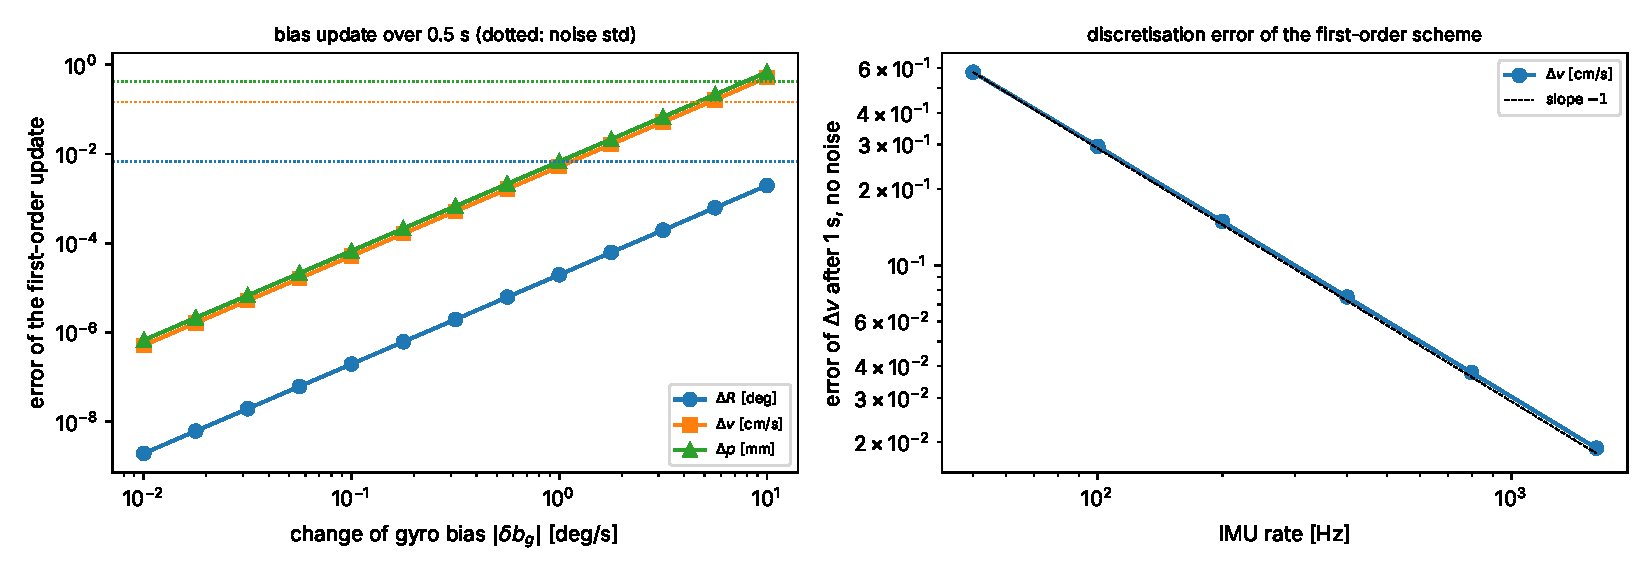
\includegraphics[width=\linewidth]{figures/ch12_bias.pdf}
\caption{Left: error of the first-order bias update
\eqref{eq:biasupd} against re-integration over 0.5\,s, as the gyroscope
bias changes; dotted: the noise standard deviations of the same
quantities. Right: error of the first-order integration scheme on the
lawn trajectory, without noise, against the IMU rate.}
\label{fig:imubias}
\end{figure}

The left of \cref{fig:imubias} shows that the error of the update grows
quadratically. It reaches the noise level only for a bias change of
about $5^\circ$/s, far more than a gyroscope bias moves within a
sliding window (its random walk, $\sigma_{bg}\sqrt{t}$, is
$0.001^\circ$/s after one second). Implementations nonetheless integrate again
(at the new linearisation point) when the change exceeds a threshold,
to keep the error well below the noise. The right of the figure is the
discretisation error of \cref{lem:imustep}: first order, 1.5\,mm/s after
1\,s at 200\,Hz, of the order of the noise.

\section{The IMU factor}

\begin{definition}{IMU factor}{imufactor}
Between keyframes $i$ and $j$, with preintegrated measurements at
linearisation biases $\bar{\vect{b}}$ and covariance $\Sigma_{ij}$, the
IMU factor has the residual
\begin{equation}\label{eq:imures}
\vect{r}_{ij}=\begin{pmatrix}
\Log\bigl(\Delta R_{ij}(\vect{b}_i)\T R_i\T R_j\bigr)\\
R_i\T(\vect{v}_j-\vect{v}_i-\vect{g}\Delta t_{ij})-\Delta\vect{v}_{ij}(
\vect{b}_i)\\
R_i\T\bigl(\p_j-\p_i-\vect{v}_i\Delta t_{ij}-\frac12\vect{g}\Delta
t_{ij}^2\bigr)-\Delta\p_{ij}(\vect{b}_i)
\end{pmatrix}
\end{equation}
with information $\Sigma_{ij}^{-1}$, the corrected measurements
\eqref{eq:biasupd} being evaluated at the biases $\vect{b}_i$ of
keyframe $i$. A \emph{bias factor} $\vect{b}_j-\vect{b}_i$ with
covariance $\diag(\sigma_{bg}^2I,\sigma_{ba}^2I)\Delta t_{ij}$
(\cref{prop:discnoise}) links the biases of successive keyframes.
\end{definition}

The residual compares the measurements with \eqref{eq:preintinv}. Its
rotation part is the error $\delta\bphi_{ij}$ of \eqref{eq:preinterr}
with a sign change, and its velocity and position parts are $-\delta
\vect{v}_{ij}$ and $-\delta\p_{ij}$; the signs do not affect the
covariance, so $\Sigma_{ij}$ is the covariance of $\vect{r}_{ij}$.

\begin{proposition}{Jacobians of the IMU factor}{imujac}
With perturbations $R\leftarrow R\Exp(\delta\bphi)$, $\vect{v}\leftarrow
\vect{v}+\delta\vect{v}$, $\p\leftarrow\p+R\,\delta\p$, $\vect{b}\leftarrow
\vect{b}+\delta\vect{b}$, write $\vect{r}_R,\vect{r}_v,\vect{r}_p$ for the
three blocks of \eqref{eq:imures}, $\Delta\vect{b}_g=\vect{b}_{g,i}-
\bar{\vect{b}}_g$, and $J_r^{-1}=J_r(\vect{r}_R)^{-1}$. The non-zero
Jacobians are
\begin{align*}
\frac{\partial\vect{r}_R}{\partial\delta\bphi_i}&=-J_r^{-1}R_j\T R_i,&
\frac{\partial\vect{r}_R}{\partial\delta\bphi_j}&=J_r^{-1},\\
\frac{\partial\vect{r}_R}{\partial\delta\vect{b}_g}&=-J_r^{-1}
\Exp(\vect{r}_R)\T J_r(J^R_{ij}\Delta\vect{b}_g)\,J^R_{ij},\\
\frac{\partial\vect{r}_v}{\partial\delta\bphi_i}&=\hatop{\bigl(R_i\T(
\vect{v}_j-\vect{v}_i-\vect{g}\Delta t_{ij})\bigr)},&
\frac{\partial\vect{r}_v}{\partial\delta\vect{b}}&=-\bigl(J^{v,g}_{ij}\;
J^{v,a}_{ij}\bigr),\\
\frac{\partial\vect{r}_v}{\partial\delta\vect{v}_i}&=-R_i\T,&
\frac{\partial\vect{r}_v}{\partial\delta\vect{v}_j}&=R_i\T,\\
\frac{\partial\vect{r}_p}{\partial\delta\bphi_i}&=\hatop{\bigl(R_i\T
\bigl(\p_j-\p_i-\vect{v}_i\Delta t_{ij}-\tfrac12\vect{g}\Delta t_{ij}^2
\bigr)\bigr)},&
\frac{\partial\vect{r}_p}{\partial\delta\vect{b}}&=-\bigl(J^{p,g}_{ij}\;
J^{p,a}_{ij}\bigr),\\
\frac{\partial\vect{r}_p}{\partial\delta\vect{v}_i}&=-R_i\T\Delta t_{ij},&
\frac{\partial\vect{r}_p}{\partial\delta\p_i}&=-I,\qquad
\frac{\partial\vect{r}_p}{\partial\delta\p_j}=R_i\T R_j .
\end{align*}
\end{proposition}

\begin{proof}
\emph{Rotation.} Let $M=\Delta R_{ij}(\vect{b}_i)\T R_i\T R_j=
\Exp(\vect{r}_R)$. Perturbing $R_j$ gives $M\Exp(\delta\bphi_j)$, and
by \cref{prop:jrinv}
\[
\Log\bigl(\Exp(\vect{r}_R)\Exp(\delta\bphi_j)\bigr)\approx
\vect{r}_R+J_r^{-1}\delta\bphi_j .
\] Perturbing $R_i$ gives
$\Delta R\T\Exp(-\delta\bphi_i)R_i\T R_j=M\Exp(-R_j\T R_i\delta\bphi_i)$ by
the second identity \eqref{eq:so3id} applied with $R=R_i\T R_j$,
whence $-J_r^{-1}R_j\T R_i$. For the bias,
$\Delta R(\vect{b}_i+\delta\vect{b}_g)=\Delta R(\bar{\vect{b}})
\Exp(J^R(\Delta\vect{b}_g+\delta\vect{b}_g))\approx\Delta R(\vect{b}_i)
\Exp(J_r(J^R\Delta\vect{b}_g)J^R\delta\vect{b}_g)$ by the first identity;
its transpose puts $\Exp(-\vect{x})$, $\vect{x}=J_r(J^R\Delta\vect{b}_g)
J^R\delta\vect{b}_g$, on the left of $M$, and $\Exp(-\vect{x})M=
M\Exp(-M\T\vect{x})$ gives the stated Jacobian.

\emph{Velocity and position.} For any vector $\vect{u}$,
$(R_i\Exp(\delta\bphi))\T\vect{u}=\Exp(-\delta\bphi)R_i\T\vect{u}\approx
R_i\T\vect{u}-\hatop{\delta\bphi}R_i\T\vect{u}=R_i\T\vect{u}+\hatop{(R_i\T
\vect{u})}\delta\bphi$, which gives the $\delta\bphi_i$ columns. The
velocity and bias columns are read off \eqref{eq:imures} and
\eqref{eq:biasupd}, which are linear in them. For the positions,
$\p_j+R_j\delta\p_j$ adds $R_i\T R_j\delta\p_j$ and $\p_i+R_i\delta\p_i$
adds $-R_i\T R_i\delta\p_i=-\delta\p_i$.
\end{proof}

The factor does not depend on $R_j$ through $\vect{r}_v$ or $\vect{r}_p$,
nor on the biases of keyframe $j$: these are linked to the rest only
through the next IMU factor and the bias factor.

\begin{mower}
An IMU on a ride-on mower lives in a harsh place. The engine and the
blades vibrate the frame at tens to hundreds of hertz, with
accelerations that can reach several $g$ and which the IMU, sampling at
200\,Hz, would alias into slow, false motion. The defence is mechanical
and electronic: mount the IMU rigidly to the camera (they must move as
one body) on vibration dampers tuned well below the vibration
frequencies, choose an accelerometer range that does not saturate, and
enable the sensor's internal anti-aliasing low-pass filter. Then record
a few hours with the engine \emph{off} for the Allan analysis, and a
few minutes with it running at full throttle to see what the vibration
adds to the noise densities. Inflating them to match is a legitimate,
and common, fix. Finally, the camera and the IMU must share a clock:
a hardware trigger or a sensor that timestamps both (as integrated
stereo--IMU modules do) avoids a time offset that Chapter~13 would
otherwise have to estimate.
\end{mower}

\begin{practice}[\code{vslam/imu.py}, \code{examples/ch12\_imu.py},
  \code{notebooks/ch12\_imu.ipynb}]
\begin{center}
\begin{tabular}{@{}ll@{}}
\toprule
Code & Formula\\
\midrule
\code{imu.ImuParams.discrete} & \cref{prop:discnoise}\\
\code{imu.simulate}, \code{lawn\_trajectory} & \eqref{eq:imumodel}\\
\code{imu.allan\_deviation} & \cref{def:allan} (overlapping)\\
\code{imu.step}, \code{dead\_reckon} & \cref{lem:imustep}\\
\code{imu.Preintegration.integrate} & \eqref{eq:preint},
  \cref{prop:preintnoise,prop:preintbias}\\
\code{.corrected}, \code{.predict} & \eqref{eq:biasupd},
  \cref{thm:preint}\\
\code{.residual}, \code{.jacobians} & \cref{def:imufactor},
  \cref{prop:imujac}\\
\bottomrule
\end{tabular}
\end{center}
The tests check that noise-free integration follows a smooth trajectory
(to the order of the scheme), that preintegration predicts exactly what
direct integration gives, the covariance of the preintegrated
measurements against 3000 Monte Carlo runs, the bias Jacobians against
re-integration, the factor Jacobians against finite differences, that
the residual vanishes at the truth, and the two Allan slopes.
\end{practice}

\section*{Further reading and C++ pointers}
\addcontentsline{toc}{section}{Further reading and C++ pointers}

Inertial navigation: D.~Titterton and J.~Weston, \emph{Strapdown
Inertial Navigation Technology}, and P.~D.~Groves, \emph{Principles of
GNSS, Inertial, and Multisensor Integrated Navigation Systems}. Allan
variance: IEEE Std 952-1997 and N.~El-Sheimy, H.~Hou and X.~Niu (IEEE
Transactions on Instrumentation and Measurement 2008). Preintegration
was introduced by T.~Lupton and S.~Sukkarieh (IEEE T-RO 2012) and put on
the manifold by C.~Forster, L.~Carlone, F.~Dellaert and D.~Scaramuzza
(IEEE T-RO 2017), whose derivation this chapter follows; K.~Eckenhoff,
P.~Geneva and G.~Huang give closed-form, higher-order versions (IJRR
2019). J.~Sol\`a's \emph{Quaternion kinematics for the error-state
Kalman filter} (2017) is a careful reference for the filtering side. In
C++: GTSAM's \code{PreintegratedImuMeasurements}, \code{ImuFactor} and
\code{CombinedImuFactor}; the IMU factors of VINS-Mono/VINS-Fusion and
OKVIS; \code{allan\_variance\_ros} and Kalibr for calibration.

\FloatBarrier
\section*{Exercises}
\addcontentsline{toc}{section}{Exercises}

\begin{enumerate}[label=\textbf{12.\arabic*},ref=12.\arabic*]
\item\label{ex:12units} Convert the EuRoC densities ($\sigma_g=1.6968
  \times10^{-4}$\,rad/s/$\sqrt{\text{Hz}}$, $\sigma_a=2.0\times10^{-3}$\,
  m/s$^2$/$\sqrt{\text{Hz}}$) to $^\circ/\sqrt{\text{h}}$ and
  $\mu g/\sqrt{\text{Hz}}$. Find the minimum of the gyroscope's Allan
  deviation in the model of \cref{prop:allanforms} ($\sigma_{bg}=1.9393
  \times10^{-5}$), and where it is reached.
\item\label{ex:12ramp} Show that a constant has zero Allan variance and
  that a ramp $y(t)=Kt$ has $\sigma_A^2(\tau)=K^2\tau^2/2$.
\item\label{ex:12tilt} A level IMU at rest reads its accelerometer. Show
  that roll and pitch are observable from it but yaw is not, and that an
  accelerometer bias $b$ along a horizontal axis causes a tilt error of
  about $b/g$. Evaluate for $b=0.02$\,m/s$^2$.
\item\label{ex:12grav} Why is gravity kept out of $\Delta\vect{v}_{ij}$
  and $\Delta\p_{ij}$ instead of being integrated with the specific force,
  and why is pulling it out as $\vect{g}\Delta t_{ij}$ exact rather than an
  approximation?
\end{enumerate}

\subsection*{Solutions}

\textbf{12.1.} $\sigma_g\cdot\frac{180}\pi\cdot60=0.58^\circ/\sqrt{\text{h}}$
(a rad/s/$\sqrt{\text{Hz}}$ is a rad/$\sqrt{\text{s}}$, and $\sqrt{3600}
=60$). $\sigma_a/9.81=2.0\times10^{-4}g$, i.e.\ $204\,\mu g/\sqrt{\text{Hz}}$.
$\sigma_A^2=\sigma_g^2/\tau+\sigma_{bg}^2\tau/3$ is minimal where its
derivative vanishes, $\sigma_g^2/\tau^2=\sigma_{bg}^2/3$, i.e.\ $\tau^*=
\sqrt3\,\sigma_g/\sigma_{bg}=15.2$\,s, where both terms are equal and
$\sigma_A=\sigma_g\sqrt{2/\tau^*}=6.2\times10^{-5}$\,rad/s, about
$13^\circ$/h (\cref{fig:allan}).

\textbf{12.2.} For a constant $c$, $\bar y_k=c$ for every $k$ and the
differences vanish. For a ramp, $\bar y_k=K(k+\frac12)\tau$, so
$\bar y_{k+1}-\bar y_k=K\tau$ and $\sigma_A^2=\frac12K^2\tau^2$: a line of
slope $+1$ on the log--log plot, which is how slow thermal drifts show up.

\textbf{12.3.} At rest $\tilde{\vect{a}}=R\T(-\vect{g})=9.81\,R\T
\vect{e}_z$: the reading is the vertical axis expressed in the body
frame, which determines roll and pitch. A rotation about the vertical,
$R\leftarrow R_z(\psi)R$, leaves $R\T\vect{e}_z$ unchanged, so yaw is not
observable. A bias $b$ along body $x$ tilts the measured vertical by an
angle $\arctan(b/g)\approx b/g$; for $0.02$\,m/s$^2$, $2.0\times10^{-3}$\,
rad $=0.12^\circ$. This is why the accelerometer bias and the tilt are
hard to separate without motion.

\textbf{12.4.} Gravity is constant in the world frame, while the
preintegrated quantities are expressed in the frame of keyframe $i$;
integrating gravity with them would require $R_i$, which is exactly
the dependence preintegration removes. And because $\vect{g}$ is
constant, its contributions $\int_{t_i}^{t_j}\vect{g}\,dt=\vect{g}
\Delta t_{ij}$ and $\iint\vect{g}=\frac12\vect{g}\Delta t_{ij}^2$ are
exact: no rotation is involved, so no approximation is made
(\cref{thm:preint}).
